\chapter{Pesquisa Bibliográfica}

A realidade humana é construída coletivamente. Não se faz ciência de forma isolada do mundo. É preciso recorrer ao conhecimento preexistente, nem que seja para criticá-lo, e a crítica faz parte da atividade de pesquisa.

O primeiro trabalho nesta disciplina compreende apresentar uma pesquisa bibliográfica usando técnicas já conhecidas, e outras mais recentemente desenvolvidas.

São várias as formas de condução de uma pesquisa bibliográfica, que também pode ser chamada de revisão da literatura.

\section{Revisão sistemática da literatura e meta-análise}

As formas mais avançadas de pesquisa bibliográfica  são as revisões sistemáticas da literatura e as meta-análises \citep{littell_systematic_2008,dresch_systematic_2015,higgins_cochrane_2011}, bastante usadas em pesquisa epidemiológica, que são feitas em grupo, com múltiplos revisores. Para uma introdução em vídeo sobre esse tema, em poucos minutos, veja \cite{testoni_revisao_2015}.

\section{Método da Análise Bibliométrica\label{metodo:analise:bibliografica}}

Focaremos, nesta disciplina, no método de análise bibliométrica, dada a sua afinidade quantitativa, que envolve o uso de ferramentas computacionais para análise de registros obtidos a partir de bases de dados de referências bibliográficas. A análise bibliométrica, ou pesquisa bibliométrica, é, portanto, uma abordagem de pesquisa empírica, eminentemente quantitativa.

Para emprego da análise bibliométrica usaremos a ferramenta Bibliometrix, e o seu \textit{workflow} de trabalho proposto, conforme aborda \cite{aria_bibliometrix_2017}, composto por cinco etapas \cite[p. 950]{aria_bibliometrix_2017}:
\begin{enumerate}
\item Study design;
\item Data collection;
\item Data analysis;
\item Data visualization;
\item Interpretation.
\end{enumerate}

Os slides usados em apoio ao conhecimento sobre o uso do Bibliometrix encontram-se no apêndice ~\ref{bibliometrix}.

Existem vários exemplos de análises bibliométricas já publicadas que usam o Bibliometrix como ferramenta principal, dentre os quais destaco os seguintes trabalhos:
\begin{enumerate}
    \item Em ``A Bibliometric Overview of Twitter-Related Studies Indexed in Web of Science'', \cite{yu_bibliometric_2020} investigam as tendências em pesquisas ligadas ao uso do Twitter, analisado a estrutura e dinâmica de 19.205 artigos acadêmicos recuperados na base Web of Science. São feitas análises de dinâmica das publicações em cinco categorias: (1) produção científica mundial, (2) fontes de informação, (3) autores, (4) publicações (\textit{papers}) e (5) palavras-chave, dentre outras análises.
    \item Em ``Scientific production and thematic breakthroughs in smart learning environments: a bibliometric analysis'', \cite{agbo_scientific_2021} investigam o ``landscape'' da pesquisa sobre ambientes \textit{smart}. Foram analisadas as tendências de pesquisa, a produtividade acadêmica, os temas focais de publicação, a partir da análise de 1081 registros bibliográficos recuperados da base SCOPUS. O artigo evidencia a importância desse tipo de estudo para dar foco às áreas de investigação dos pesquisadores iniciantes nessa área.
    \item Em ``Knowledge mapping of microfinance performance research: a bibliometric analysis'', \cite{akter_knowledge_2021} investigam as principais pesquisas relacionadas com o tema  ``desempenho de microfinanças'', evidenciado-se, entre outros aspectos, que os temas de pesquisa mais frequentes são: \textit{alívio da pobreza}, \textit{empréstimo em grupo}, \textit{escore de crédito}.
\end{enumerate}

Em todos os três estudos observa-se a utilização dos vários recursos analíticos suportados pelo pacote Bibliometrix.

\subsection{Projeto da pesquisa (\textit{study design})} 

Conforme apresenta \cite[p. 960]{aria_bibliometrix_2017},

\begin{itquote}
    In study design, scholars define the research question(s) and choose the appropriate bibliometric methods that can
answer the question(s).
\end{itquote}

\subsubsection{Pergunta de pesquisa}
A pergunta ou questão de pesquisa, ou o conjunto das questões de pesquisa, é quem deve orientar o início de todo processo de pesquisa. Nenhuma pesquisa pode avançar sem uma declaração prévia das perguntas ou questões que busca responder, sob risco de ser apenas especulativa, pois a tendência é que sejam modificados os objetivos conforme avançam os estágios subsequentes, e assim introduzindo viés no trabalho.


É natural que a pesquisa mude, mas a mudança deve ocorrer primeiramente na pergunta. Assim sendo, o ciclo da pesquisa progride de forma iterativa, como ilustra a figura ~\ref{fig:ciclo_projeto}.

Note que a pergunta de pesquisa é mais ampla, e resulta de inquietações na cabeça do pesquisador, que podem permanecer pelo resto de sua vida, enquanto que os objetivos da pesquisa são mais focados, e relacionados ao que é viável ser feito no escopo de um projeto, que tem tempo limitado para ser executado.

\begin{figure}
    \centering
    \includegraphics[page=6,width=\textwidth,clip,trim={2.0cm 3cm 2.0cm 16.3cm}]{2-Analise-Exploratoria-Dados/aulas/2.2-Pesquisa-Bibliografica/GSIC905-V1TextoBase.pdf}
    \caption{O papel do projeto de pesquisa na produção do conhecimento científico. Fonte \cite[p.6]{lopez_diretrizes_2010}}
    \label{fig:ciclo_projeto}
\end{figure}


\subsubsection{Tipos de pergunta de pesquisa em uma pesquisa bibliométrica}

Conforme [p. 960]\cite{aria_bibliometrix_2017},

\begin{itquote}

    Three general types of research questions can be answered using bibliometrics for science mapping:
    
    (i) identifying the knowledge base of a topic or research field and its intellectual structure; 
    
    (ii) examining the research front (or conceptual structure) of a topic or research field; and 

    (iii) producing a social network structure of a particular scientific
community.

\end{itquote}

Alguns esclarecimentos sobre os três focos de pergunta indicados:
\begin{enumerate}
    \item A base de conhecimentos é o conjunto de conhecimentos científicos e tecnológicos registrados e disponíveis para consulta e uso pela sociedade;
    \item O conhecimento científico está usualmente presente na forma de artigos científicos, publicados em revistas científicas;
    \item O conhecimento tecnológico está usualmente presente nas bases de patentes registradas junto aos órgãos de proteção à propriedade intelectual dos vários países;
    \item Existem outras formas e conhecimento, além do científico e tecnológico, como o religioso, cultural etc. Focaremos apenas no conhecimento científico;
    \item As bases de conhecimento estão registradas e disponíveis para uso nas bibliotecas e nos sítios web. As bases de conhecimento são \textbf{referenciadas} nas bases bibliográficas, como nos fichários de bibliotecas, ou nas bases de dados online, como Web of Science, SCOPUS, Google Acadêmico. Existem milhares de bases de dados bibliográficas no mundo inteiro, usualmente organizadas por temas, e uma lista delas pode ser vista em \url{https://en.wikipedia.org/wiki/List_of_academic_databases_and_search_engines}. 
    \item A construção e manutenção de uma base bibliográfica requer um esforço de vários profissionais dedicados, ao longo de vários anos, e o profissional da biblioteconomia é geralmente o que reúne conhecimentos sobre a questão. Nesta disciplina, o seu estudo bibliométrico vai criar e utilizar uma base, de forma bem inicial. O seu relatório vai ser um documento descritivo da sua base;
    \item A \textbf{estrutura intelectual do conhecimento} em um determinado campo é a estrutura dos relacionamentos estabelecidos durante a produção do conhecimento nesse campo, e é possível de ser evidenciada a partir a análise citações entre os artigos, escritos por autores, filiados a organizações. Por exemplo, se um artigo A cita outros tantos artigos X, Y e Z, é de se supor que a produção do conhecimento em A dependeu dos conhecimentos em X, Y e Z. Esse conjunto de relações, que formam um grafo temporalmente ordenado, é a base de representação e análise da estrutura do conhecimento subjacente. Para análise da estrutura de conhecimento, é necessário usar uma base de citações, como é o caso das bases SCOPUS e Web of Science. Nem toda base é uma base de citações (\textit{citation index}), e quando fazendo download no SCOPUS ou WoS é preciso explicitar que se quer fazer o download das citações, junto com as referências;
    \item A ``frente de pesquisa'' ou estrutura conceitual é representada principalmente pelo conjunto dos termos (palavras-chave) mais evidentes que lideram o processo de publicação do conhecimento, ou seus \textit{trending topics};
    \item Uma comunidade científica é uma rede mais ou menos fechada e dinâmica, representada por um ou mais grafos, onde os vértices podem ser pessoas, organizações e eventos, e as arestas podem ser colaborações (em artigos, em trocas de mensagens) e co-participações (em eventos científicos).
\end{enumerate}

O trabalho a ser realizado, de forma simplificada nessa atividade na disciplina, envolve  formular perguntas inicialmente simples, que expressem a busca por cada um dos três tipos de objetivos.

\begin{enumerate}
\item Identificação da base de conhecimentos de um tópico de pesquisa e sua estrutura intelectual

\item Exame da estrutura conceitual de um tópico de pesquisa

\item Investigando a estrutura social da comunidade que produz pesquisa em um tópico específico
\end{enumerate}

Veja exemplo de perguntas de pesquisa no exemplo a ser ofertado na query em \ref{query}.

\subsection{Definição do método da pesquisa}

Usaremos a ferramenta e o \textit{workflow} proposto pelos autores do pacote Bibliometrix, para a realização do trabalho, conforme indica a figura ~\ref{fig:bibliometrix:workflow}.

\begin{figure}
    \centering
\includegraphics[page=4,width=\textwidth,clip,trim={1cm 0.6cm 1cm 9cm}]{2-Analise-Exploratoria-Dados/aulas/2.2-Pesquisa-Bibliografica/R-RStudio-Bibliometrix.pdf}
    \caption{Workflow de trabalho com Bibliometrix. Fonte: \citep{aria_bibliometrix_2017}.\label{fig:bibliometrix:workflow}}
    
\end{figure}

Como se trata de um estudo exploratório analítico, serão realizados os três passos no exercício 1, para concluir uma uma interpretação dos dados e mapas gerados.
\begin{enumerate}
    \item Coleta de dados (escolha da base, formulação e refinamento da query de busca, download dos registros, carga e conversão dos registros no Biblioshiny etc);
    \item Análise dos dados (análise descritiva, criação e descrição da matriz de atributos normalizados, redução de dados por meio de clusterização, geração da matriz em rede (grafo) com extração de métricas de grafo)
    \item Geração de mapas e gráficos
\end{enumerate}

A interpretação não é apresentada na figura \ref{fig:bibliometrix:workflow}, pois é feita pelo autor da análise, usando processos cognitivos que evidenciam a sua capacidade de interpretação objetiva e subjetiva, resultantes do tempo que dedicou-se a refletir sobre o assunto.

\section{Coleta de dados}

Conforme \cite{aria_bibliometrix_2017},
na coleta de dados 

\begin{itquote}
    scholars select the database that contains the bibliometric data, filter the core document set, and export
the data from the selected database. This step can involve constructing one’s own database (Waltman, 2016).
\end{itquote}

No caso específico dessa disciplina:
\begin{enumerate}
    \item A base de dados será da Web of Science ou SCOPUS, devido ao escopo e qualidade dadas bases;
    \item As filtragens são definidas por \textit{strings} de busca como ilustram as linhas 1 a 10 do código a seguir, usado em busca no WoS:
\lstinputlisting[numbers=left,basicstyle=\normalsize\ttfamily,caption={Anotações feitas durante uma pesquisa em base bibliográfica},label=query20210727]
{experiments/jhcf/PesqBibliogr/SimulacaoMultiagente/WoS-20210727/query.txt}

\item As bases de dados usadas na análise, assim como todo o código fonte \LaTeX~ do texto que relata a análise, devem ser armazenadas nos ambientes de experimento de cada um dos alunos, mantidos a partir do diretório \texttt{experiments/$<$githubusername$>$}, onde $<$githubusername$>$ é o username do(a) aluno(a).

\end{enumerate}

Observe, na listagem \ref{query20210727}, que a query retornou 6.105 registros, e foi feita apenas nas coleções \texttt{SCI-EXPANDED} e \texttt{SSCI}.

No seu trabalho você necessitará descrever a sua coleta de dados de forma detalhada o suficiente para que o leitor consiga obter exatamente os mesmos registros que você obteve, caso a busca fosse feita no mesmo dia em que você fez.

Para chegar a um resultado aceitável pode ser necessário executar dezenas de buscas, procurando por variações até que tenha uma melhor certeza de que quantidade e qualidade dos dados retornados reflita a busca que você deseja realizar.
É importante consultar um Thesaurus, para usar sinônimos durante a formulação das buscas. Ver um exemplo em \url{http://vocabularies.unesco.org/browser/thesaurus/en/page/?uri=http://vocabularies.unesco.org/thesaurus/concept450}.


Justifique, na apresentação de sua query, porque usou cada um dos termos apresentados na query.

\section{Análise dos dados}

conforme \cite{aria_bibliometrix_2017}, 
\begin{itquote}
one or more bibliometric or statistical software tools are employed. Alternatively, scholars can write
their own computer code to meet their requirements.    
\end{itquote}
Nesta turma, usaremos o pacote Bibliometrix com a interface Biblioshiny, que evitará a necessidade de escrita de código, nesse momento da disciplina.
Em trabalhos subsequentes, a biblioteca poderá ser integrada com a escrita de código em R.

A análise dos dados deve fazer, necessariamente:
\begin{enumerate}
    \item Uma análise bibliográfica descritiva;
    \item Uma análise bibliométrica que aplicando pelo menos duas métricas a cada um dos três níveis de análise possíveis:
    \begin{enumerate}
        \item fontes de informação;
        \item autores;
        \item documentos;
    \end{enumerate}
    \item uma análise infométrica que utilize pelo menos cinco diferentes tipos de gráficos para investigar a:
    \begin{itemize}
        \item Estrutura social do conhecimento no tópico de interesse do investigador;
        \item Estrutura Conceitual do conhecimento no tópico de interesse do investigador.
    \end{itemize}
    
\end{enumerate}

Todas as análises, na forma de tabelas e gráficos, devem ser apresentadas por texto que a acompanha.

\section{Visualização de dados}

conforme \cite{aria_bibliometrix_2017}
\begin{itquote}
Scholars must decide what visualization method is to be used on the results of the
third step and then employ the appropriate mapping software    
\end{itquote}

Todos os gráficos de subsídio às análises, escolhidos no item anterior,  devem ser apresentados e descritos cuidadosamente, tendo por objetivo de subsidiar  análise do autor, feita no próximo passo. 

\section{Interpretação dos dados}

Uma interpretação do conjunto dos dados deve evidenciar a capacidade do autor e usar as informações apresentadas para evidenciar que consegui responder às perguntas de pesquisa formuladas no início do trabalho.


